%% LyX 2.3.6.1 created this file.  For more info, see http://www.lyx.org/.
%% Do not edit unless you really know what you are doing.
\documentclass[11pt,american,czech]{book}
\usepackage[T1]{fontenc}
\usepackage[utf8]{inputenc}
\usepackage[a4paper]{geometry}
\geometry{verbose,tmargin=4cm,bmargin=3cm,lmargin=3cm,rmargin=2cm,headheight=0.8cm,headsep=1cm,footskip=0.5cm}
\pagestyle{headings}
\setcounter{secnumdepth}{3}
\usepackage{url}
\usepackage{amsmath}
\usepackage{amsthm}
\usepackage{amssymb}
\usepackage{graphicx}
\usepackage{setspace}

\makeatletter
%%%%%%%%%%%%%%%%%%%%%%%%%%%%%% Textclass specific LaTeX commands.
\newenvironment{lyxlist}[1]
	{\begin{list}{}
		{\settowidth{\labelwidth}{#1}
		 \setlength{\leftmargin}{\labelwidth}
		 \addtolength{\leftmargin}{\labelsep}
		 \renewcommand{\makelabel}[1]{##1\hfil}}}
	{\end{list}}

%%%%%%%%%%%%%%%%%%%%%%%%%%%%%% User specified LaTeX commands.
%% Font setup: please leave the LyX font settings all set to 'default'
%% if you want to use any of these packages:

%% Use Times New Roman font for text and Belleek font for math
%% Please make sure that the 'esint' package is turned off in the
%% 'Math options' page.
\usepackage[varg]{txfonts}

%% Use Utopia text with Fourier-GUTenberg math
%\usepackage{fourier}

%% Bitstream Charter text with Math Design math
%\usepackage[charter]{mathdesign}

%%---------------------------------------------------------------------

%% Make the multiline figure/table captions indent so that the second
%% line "hangs" right below the first one.
%\usepackage[format=hang]{caption}

%% Indent even the first paragraph in each section
\usepackage{indentfirst}

%%---------------------------------------------------------------------

%% Disable page numbers in the TOC. LOF, LOT (TOC automatically
%% adds \thispagestyle{chapter} if not overriden
%\addtocontents{toc}{\protect\thispagestyle{empty}}
%\addtocontents{lof}{\protect\thispagestyle{empty}}
%\addtocontents{lot}{\protect\thispagestyle{empty}}

%% Shifts the top line of the TOC (not the title) 1cm upwards 
%% so that the whole TOC fits on 1 page. Additional page size
%% adjustment is performed at the point where the TOC
%% is inserted.
%\addtocontents{toc}{\protect\vspace{-1cm}}

%%---------------------------------------------------------------------

% completely avoid orphans (first lines of a new paragraph on the bottom of a page)
\clubpenalty=9500

% completely avoid widows (last lines of paragraph on a new page)
\widowpenalty=9500

% disable hyphenation of acronyms
\hyphenation{CDFA HARDI HiPPIES IKEM InterTrack MEGIDDO MIMD MPFA DICOM ASCLEPIOS MedInria}

%%---------------------------------------------------------------------

%% Print out all vectors in bold type instead of printing an arrow above them
\renewcommand{\vec}[1]{\boldsymbol{#1}}

% Replace standard \cite by the parenthetical variant \citep
%\renewcommand{\cite}{\citep}

\makeatother

\usepackage{babel}

\def\NameOfThesisCzech{Robustní strojové učení a adversariální vzorky}
\def\NameOfThesisEnglish{Robust machine learning and adversarial examples}
\def\NameOfAuthor{Pavel Jakš}
\def\NameOfSupervisor{Mgr. Lukáš Adam, Ph.D.}

\begin{document}
\def\documentdate{7. \v{c}ervence 2022}

%%\def\documentdate{\today}

\pagestyle{empty}
{\centering

\noindent %
\begin{minipage}[c]{3cm}%
\noindent \begin{center}

\includegraphics[width=3cm,height=3cm,keepaspectratio]{Images/TITLE/cvut}
\par\end{center}%
\end{minipage}%
\begin{minipage}[c]{0.6\linewidth}%
\begin{center}
\textsc{\large{}České vysoké učení technické v Praze}{\large{}}\\
{\large{}Fakulta jaderná a fyzikálně inženýrská}
\par\end{center}%
\end{minipage}%
\begin{minipage}[c]{3cm}%
\noindent \begin{center}
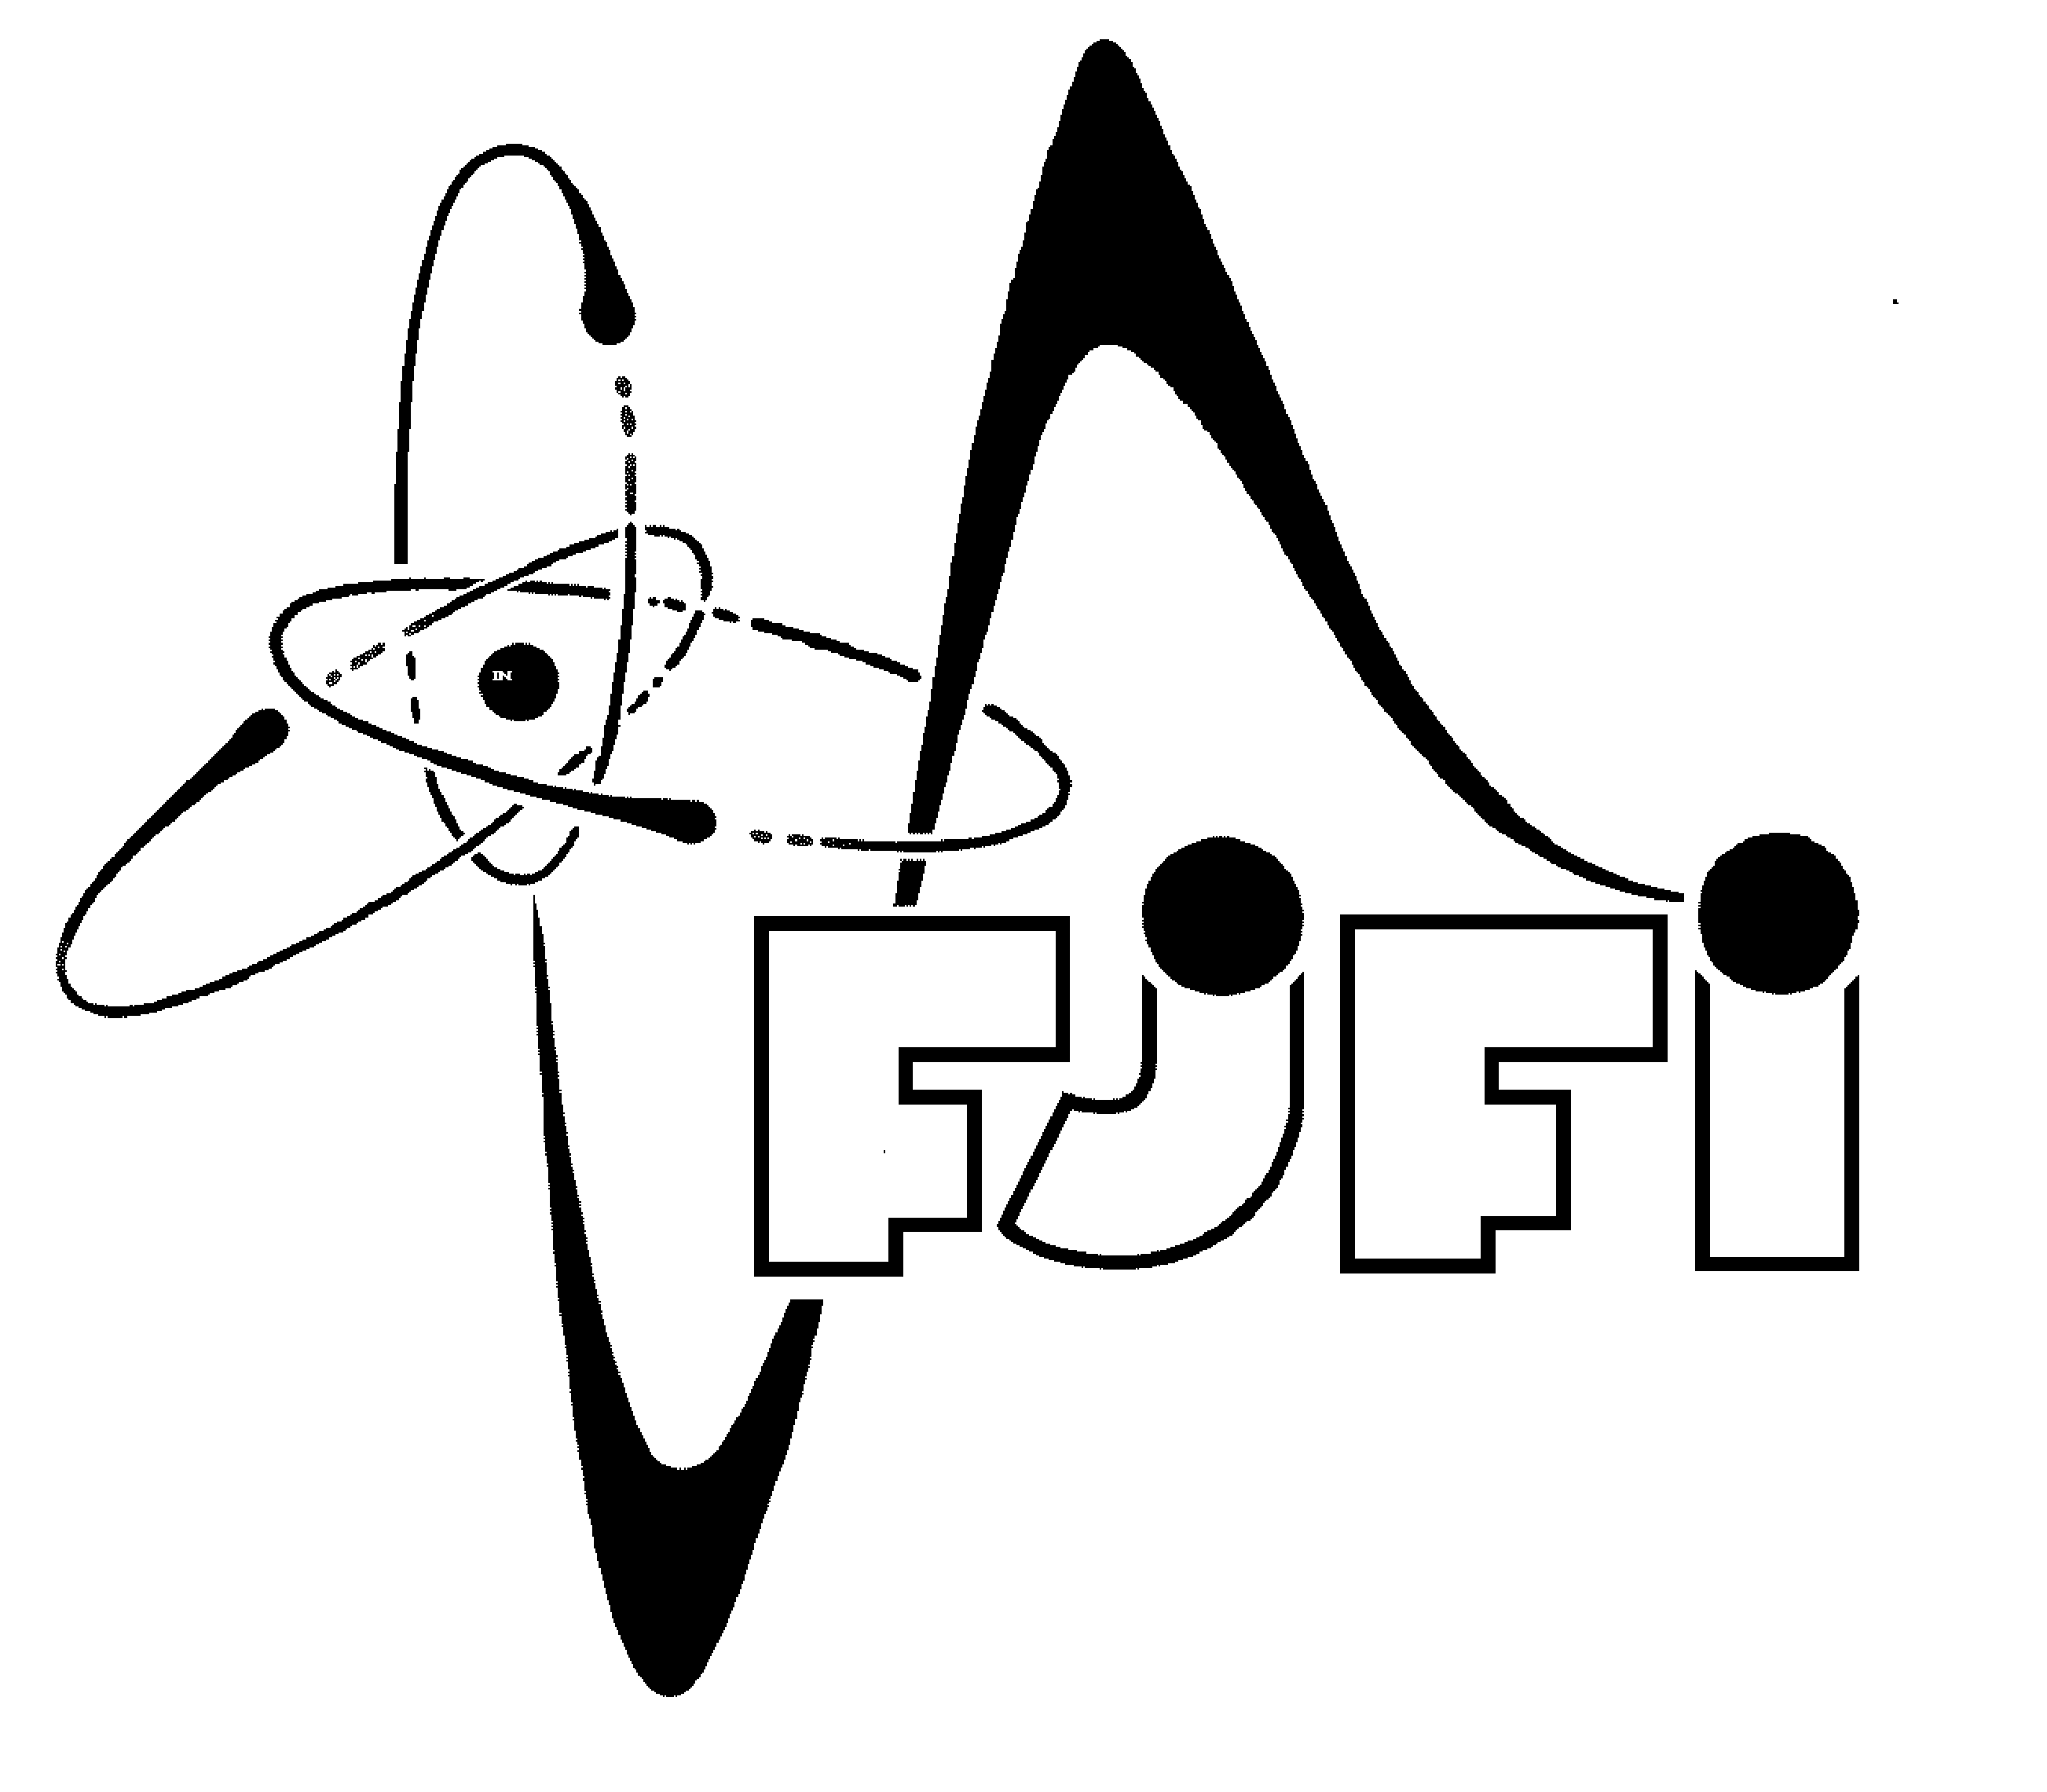
\includegraphics[width=3cm,height=3cm,keepaspectratio]{Images/TITLE/fjfi}
\par\end{center}%
\end{minipage}

\vspace{3cm}

\textbf{\huge{}\NameOfThesisCzech}{\huge\par}

\vspace{1cm}

\selectlanguage{american}%
\textbf{\huge{}\NameOfThesisEnglish}{\huge\par}

\selectlanguage{czech}%
\vspace{2cm}

{\large{}Bakalářská práce}{\large\par}

}

\vfill{}

\begin{lyxlist}{MMMMMMMMM}
\begin{singlespace}
\item [{Autor:}] \textbf{\NameOfAuthor}
\item [{Vedoucí~práce:}] \textbf{\NameOfSupervisor}
%\item [{Konzultant:}] \textbf{doc. RNDr. Jméno Konzultanta, CSc. }(pouze pokud konzultant byl jmenován.)
\item [{Akademický~rok:}] 2021/2022
\end{singlespace}
\end{lyxlist}
\newpage{}

~\newpage{}

~

\vfill{}

\begin{center}
- Zadání práce -
\par\end{center}

\vfill{}

~\newpage{}

~

\vfill{}

\begin{center}
- Zadání práce (zadní strana) -
\par\end{center}

\vfill{}

~\newpage{}

\noindent \emph{\Large{}Poděkování:}{\Large\par}

\noindent Chtěl bych zde poděkovat především svému školiteli - panu doktoru Adamovi -
za pečlivost, ochotu, vstřícnost a odborné i lidské zázemí při vedení
mé bakalářské práce.

\vfill

\noindent \emph{\Large{}Čestné prohlášení:}{\Large\par}

\noindent Prohlašuji, že jsem tuto práci vypracoval samostatně a uvedl
jsem všechnu použitou literaturu.

\bigskip{}

\noindent V Praze dne \documentdate\hfill{}\NameOfAuthor

\vspace{2cm}

\newpage{}

~\newpage{}

\begin{onehalfspace}
\noindent \emph{Název práce:}

\noindent \textbf{\NameOfThesisCzech}
\end{onehalfspace}

\bigskip{}

\noindent \emph{Autor:} \NameOfAuthor

\bigskip{}

\noindent \emph{Obor:} Matematická informatika\bigskip{}

% \noindent \emph{Zaměření:} Celý název zaměření (Pokud obor neobsahuje zaměření, tuto řádku odstranit.)

\bigskip{}

\noindent \emph{Druh práce:} Bakalářská práce

\bigskip{}

\noindent \emph{Vedoucí práce:} \NameOfSupervisor,
Katedra počítačů,
Fakulta elektrotechnická,
České vysoké učení technické v Praze,
Karlovo náměstí 13, 121 35, Praha 2

\bigskip{}

% \noindent \emph{Konzultant:} doc. RNDr. Jméno Konzultanta, CSc., pracoviště
% konzultanta. Pouze pokud konzultant byl jmenován.

\bigskip{}

\noindent \emph{Abstrakt:} Abstrakt max. na 10 řádků. Abstrakt max.
na 10 řádků. Abstrakt max. na 10 řádků. Abstrakt max. na 10 řádků.
Abstrakt max. na 10 řádků. Abstrakt max. na 10 řádků. Abstrakt max.
na 10 řádků. Abstrakt max. na 10 řádků. Abstrakt max. na 10 řádků.
Abstrakt max. na 10 řádků. Abstrakt max. na 10 řádků. Abstrakt max.
na 10 řádků. Abstrakt max. na 10 řádků. Abstrakt max. na 10 řádků.
Abstrakt max. na 10 řádků. Abstrakt max. na 10 řádků. Abstrakt max.
na 10 řádků. Abstrakt max. na 10 řádků. Abstrakt max. na 10 řádků.
Abstrakt max. na 10 řádků. Abstrakt max. na 10 řádků. Abstrakt max.
na 10 řádků. Abstrakt max. na 10 řádků. Abstrakt max. na 10 řádků.
Abstrakt max. na 10 řádků. Abstrakt max. na 10 řádků. Abstrakt max.
na 10 řádků. Abstrakt max. na 10 řádků. Abstrakt max. na 10 řádků. 

\bigskip{}

\noindent \emph{Klíčová slova:} klíčová slova (nebo výrazy) seřazená
podle abecedy a oddělená čárkou

\vfill{}
~

\selectlanguage{american}%
\begin{onehalfspace}
\noindent \emph{Title:}

\noindent \textbf{\NameOfThesisEnglish}
\end{onehalfspace}

\bigskip{}

\noindent \emph{Author:} \NameOfAuthor

\bigskip{}

\noindent \emph{Abstract:} Max. 10 lines of English abstract text.
Max. 10 lines of English abstract text. Max. 10 lines of English abstract
text. Max. 10 lines of English abstract text. Max. 10 lines of English
abstract text. Max. 10 lines of English abstract text. Max. 10 lines
of English abstract text. Max. 10 lines of English abstract text.
Max. 10 lines of English abstract text. Max. 10 lines of English abstract
text. Max. 10 lines of English abstract text. Max. 10 lines of English
abstract text. Max. 10 lines of English abstract text. Max. 10 lines
of English abstract text. Max. 10 lines of English abstract text.
Max. 10 lines of English abstract text. Max. 10 lines of English abstract
text. Max. 10 lines of English abstract text. Max. 10 lines of English
abstract text. Max. 10 lines of English abstract text. Max. 10 lines
of English abstract text. Max. 10 lines of English abstract text.
Max. 10 lines of English abstract text. Max. 10 lines of English abstract
text. Max. 10 lines of English abstract text.

\bigskip{}

\noindent \emph{Key words:} keywords in alphabetical order separated
by commas

\selectlanguage{czech}%
\newpage{}

~\newpage{}

\pagestyle{plain}

\tableofcontents{}

\newpage{}

\chapter*{Úvod}

\addcontentsline{toc}{chapter}{Úvod}

Pojem neuronové sítě představuje výpočetní jednotku, která svou univerzálností nachází uplatnění v~mnoha disciplínách.

% Neuronové sítě
\chapter{Neuronové sítě}

% Úvodní pojednání o neuronových sítích
% Umělý neuron
Princip fungování neuronové sítě spočívá v poskládání celku z dílčích výpočetních jednotek - umělých neuronů.
Takovýto neuron je standardně funkcí více proměnných, jehož výstup je proměnná jediná.
Typickým modelem umělého neuronu je funkce $f: \mathbb{R}^n \rightarrow \mathbb{R}$ definovaná předpisem
\begin{equation} \label{neuron}
	f(a_1, ..., a_n) = \sigma (\sum_{i=1}^n w_i a_i + b) ,
\end{equation}
kde \emph{n} je počet vstupujících proměnných, \emph{$w_i$} jsou tzv. váhy (w z anglického slova weight),
\emph{b} je práh (b~z~anglického slova bias), \emph{$\sigma$} označuje tzv. aktivační funkci.

Roli vstupujících proměnných mohou hrát např. hodnoty RGB pixelů barevných obrázků, je-li aplikací klasifikace obrázků,
nebo výstupy jiných neuronů.
Pod pojmem váha se skrývá míra ovlivnění výstupu neuronu daným vstupem.
Je-li váha u nějakého vstupu vysoká, pak je výstup citlivější na daný vstup.
Práh pro změnu určuje posunutí citlivosti neuronu na všechny vstupy jako celku.

Poslední, avšak velmi důležitou charakteristikou tohoto modelu neuronu je aktivační funkce.
Za aktivační funkci lze vzít libovolnou funkci $\sigma : \mathbb{R} \rightarrow \mathbb{R}$,
existuje však základní sada:
\begin{itemize}
	\item Sigmoid: $\sigma(z) = \frac{1}{1 + e^{-z}}$
	\item ReLU: $\sigma(z) = max(0, z)$
	\item LeakyReLU: $\sigma(z) = max(0, z) + \alpha * min(z, 0)$, kde $\alpha \in \mathbb{R}^+$
	\item Tanh: $\sigma(z) = tanh(z) = \frac{e^{z} - e^{-z}}{e^{z} + e^{-z}}$
\end{itemize}
Tyto funkce lze doplnit o jejich mírné modifikace.
Moderní doporučenou praxí je užívat ReLU jako aktivační funkci a (\ref{neuron}) jako model neuronu dle \cite{Goodfellow}.


\section{Hluboká dopředná neuronová síť}
Je-li pojem umělého neuronu objasněn, lze se přesunout k jeho užití v neuronových sítích.
Základní myšlenkou těchto sítí je vhodné poskládání umělých neuronů do vrstev, které dohromady tvoří síť neuronů.
Taková vrstva je potom trojího druhu - vstupní, výstupní a skrytá.
\emph{Vstupní vrstva} je množina umělých neuronů, které mají za vstup výstupy problému, jehož je neuronová síť řešením.
Za vstup si lze představit matici černobílých pixelů, které představují obrázek číslice, kterou je cíl klasifikovat.
\emph{Výstupní} vrstva sestává z neuronů, které mají za vstup výstupy neuronů předchozí vrstvy.
Výstupem této vrstvy pak bude řešení daného problému - například klasifikace číslice.
Posledním druhem vrstvy je \emph{vrstva skrytá}.
Takováto vrstva má za vstupy výstupy vrstvy předcházející a její výstupy slouží jako vstupy pro~vrstvu nadcházející.
Má-li neuronová síť tuto architekturu, hovoří se o \emph{dopředné neuronové síti}.
Má-li navíc alespoň jednu skrytou vrstvu, lze mluvit o \emph{hluboké dopředné neuronové síti}.

Se znalostí pojmu vrstvy neuronů lze přistoupit k poznámce o tzv. \emph{softmax funkci}.
Jedná se o vektorovou funkci $s: \mathbb{R}^m \rightarrow \mathbb{R}^m$, kde
\begin{equation*}
	s(a_1, ..., a_m)_i = \frac{e^{a_i}}{\sum_{j=1}^m e^{a_j}},
\end{equation*}
kde $i \in \hat{m}$.
Její užití je nasnadě: Výstup této funkce lze totiž interpretovat jako diskrétní pravděpodobnostní distribuci,
a proto ji lze užít jako aktivační funkci výstupní vrstvy, je-li cílem dané neuronové sítě klasifikace vstupu do kategorií.

Další poznámka se bude věnovat zjednodušení zápisu akce vrstvy na vstup.
Podle modelu neuronu v~(\ref{neuron}) se akce jednodnoho neuronu na vstup sestává z násobení,
následného sčítání, přičtení prahu a aplikací aktivační funkce.
Tato procedura nastává pro každý neuron ve vrstvě.
Tak lze sestavit z jednotlivých vah $w_i^{(j)}$ (\emph{i}-tá váha \emph{j}-tého neuronu ve vrstvě) matici $\mathbb{A}$,
jejímiž prvky jsou právě ony váhy $(\mathbb{A})_{j,i} = w_i^{(j)}$,
z~prahů pak vektor $b$, jehož $j$-tá složka je rovna prahu $j$-tého neuronu.
Dále zaveďme vektorovou funkci $s: \mathbb{R}^m \rightarrow \mathbb{R}^m$ - ať už jako výše zmíněnou softmax funkci,
nebo jako po složkách aplikovanou libovolnou aktivační funkci $\sigma$
ve smyslu $s(a_1, ... a_m)_i = \sigma(a_i)$ pro $i \in \hat{m}$. 
Pak lze psát, že aplikace vrstvy neuronů je zobrazení $\phi : \mathbb{R}^n \rightarrow \mathbb{R}^m$
působící na vektor $a$ následovně:
\begin{equation} \label{layer}
	\phi(a) = s(\mathbb{A}a + b)
\end{equation}
Tedy stěžejní operací se stává maticové násobení, respektive násebení vektoru maticí zprava.

Při tomto si lze povšimnout, že takováto neuronová síť má řadu parametrů, o kterých není jasné jak je správně nastavit.
Některé parametry (například váhy a prahy) se nastavují během učení neuronové sítě, čemuž je věnována samostatná kapitola.
Potom tu jsou parametry, jejichž charakter je poněkud odlišný.
Jedná se o ty parametry, které zůstávají během života neuronové sítě netknuté.
Jako příklad lze uvést počet neuronů ve skryté vrstvě, který se promítne v rozměrech matice vah či dimenzionalitě výstupu vrstvy.
Takovýmto prametrům je přisuzován název hyper-parametry.

\section{Konvoluční sítě}

% Úvod do CNNs
\emph{Konvoluční sítě} nebo též \emph{konvoluční neuronové sítě} přinášejí svou architekturou
nové možnosti zpracování dat se specifickou strukturou, do které patří například časové řady,
obrázky nebo videa.
Středobodem konvolučních sítí je, jak již název napovídá, operace \emph{konvoluce}.
Ta nahrazuje maticové násobení, kterým lze reprezentovat operace ve výše popsaném modelu hluboké dopředné sítě.

% \subsection{Konvoluce}

Operace \emph{konvoluce} je ve vší obecnosti operace mezi dvěma číselnými funkcemi $g$ a $h$ se stejným definičním oborem,
jejíž výstupem je nová číselná funkce standardně označovaná jako $g*h$.
Uveďme zde definici konvoluce pro reálné funkce definované na $\mathbb{R}^d$,
tedy $g,h: \mathbb{R}^d \rightarrow \mathbb{R}$:
\begin{equation*}
	(g * h)(t) = \int_{\mathbb{R}^{d}} g(\tau) h(t - \tau) d\tau
\end{equation*}
Důležitým předpokladem pro možnost konvoluce je samozřejmě konvergence integrálu na pravé straně.

Ačkoliv je konvoluce komutativní operací, v kontextu strojového učení se mezi oběma funkcemi vstupujícími do konvoluce rozlišuje.
Funkce vstupující jako první se nazývá vstup a druhá funkce se nazývá jádrem.
Dále se v kontextu konvolučních sítí standardně objevují diskrétní funkce,
které nabývají nenulových hodnot pouze v konečně mnoha bodech.
Potom integrál přes $\mathbb{R}^d$ přechází v konečnou sumu:
\begin{equation}
	(g * h)(i_1, ..., i_d) = \sum_{j_1} ... \sum_{j_d} g(j_1, ..., j_d) h(i_1 - j_1, ..., i_d - j_d)
\end{equation}
Díky komutativitě konvoluce lze též psát:
\begin{equation}
	(g * h)(i_1, ..., i_d) = \sum_{j_1} ... \sum_{j_d} g(i_1 - j_1, ..., i_d - j_d) h(j_1, ..., j_d)
\end{equation}
Při aplikaci komutativity došlo k tzv. \emph{překlopení jádra} (termín pochází z anglického kernel flipping).
Za~vynechání překlopení jádra lze dojít ke \emph{křížové korelaci}:
\begin{equation}
	(g * h)(i_1, ..., i_d) = \sum_{j_1} ... \sum_{j_d} g(i_1 + j_1, ..., i_d + j_d) h(j_1, ..., j_d)
\end{equation}
Mnoho knihoven zabývajících se neuronovými sítěmi dle \cite{Goodfellow} implementují křížovou korelaci namísto konvoluce,
ačkoliv tuto svou implementaci nazývají konvolucí.

% \subsection{Pooling}
Další nedílnou součástí konvolučních sítí je tzv. \emph{pooling}.
Spolu s konvolucí tvoří mocný nástroj, který ve formě konvolučních a pooling vrstev hlubokých neuronových sítí
přináší například invarianci sítě vůči malému posunutí vstupu (dle \cite{Goodfellow}).

Pooling je funkce, která nahrazuje hodnoty v bodech nějakou souhrnou statistikou určitého okolí daného bodu.
Např. \emph{max pooling} aplikovaný na matici se podívá na obdélníkové okolí předem definovaných rozměrů daného bodu
a jako svůj výstup vybere maximální hodnotu nalezenou v onom okolí.
Jiné oblíbené pooling funkce zahrnují funkce reportující průměr či $L^2$ normu daného obdelníkového okolí.

Standardní konvoluční vrstva neuronové sítě pak sestává ze tří fází.
První fáze provádí paralelně několik konvolucí, které produkují sadu aktivcí.
Druhá fáze, někdy označovaná jako \emph{detekční fáze}, aplikuje na výstupy první fáze aktivační funkci.
Třetí fáze potom provádí \emph{pooling}.

% Dle \cite{Goodfellow} pooling přidává neuronové síti tu vlastnost, že je \emph{invariantní vůči malým translacím} na vstupu.
% Tj. dojde-li k posunutí hodnot vstupu o malou hodnotu, díky poolingu dojde ke změně výstupu konvoluční vrstvy jen v malém počtu výstupů.

% Učení neuronové sítě
\chapter{Učení neuronové sítě}

Standardní přístup k \emph{učení neuronové sítě}, což je termín,
kterým se označuje vhodné nalezení parametrů neuronové sítě,
je paradigma učení s učitelem.
Tento pohled na učení neuronové sítě předpokládá existenci
tzv. \emph{trénovací sady dat} $\mathbb{T}$ (angl. \emph{training dataset}),
což je uspořádaná dvojice obsahující množinu \emph{vzorků} $\mathbb{X} = \{x^{(i)} | i \in \hat{N} \}$
a k nim příslušné \emph{značky} $\mathbb{Y} = \{y^{(i)} | i \in \hat{N} \}$,
kde pojem vzorek představuje vstup neuronové sítě jakožto zobrazení
a pojem značka představuje správný výstup neuronové sítě;
$N$ je potom velikost trénovací sady $\mathbb{T}$.
Trénovací sada pak hraje roli učitele.

% Předchozí kapitola představuje neuronové sítě jakožto složené zobrazení s mnoha parametry.
% Aby takováto neuronová síť byla k něčemu užitečná, např. ke klasifikaci obrázků, musí dané zkonstruované zobrazení
% vracet smysluplné výsledky k daným vstupům.
% Toho se v praxi dociluje vhodným nastavením hyper-parametrů sítě a následným nalezením hodnot parametrů daného složeného zobrazení,
% které odpovídají funkční neuronové síti.
% Toto hledání parametrů se též nazývá jako \emph{učení neuronové sítě}
% a provádí se metodami numerické optimalizace jistého vhodně zvoleného kritéria,
% které se označuje jako \emph{účelová} či \emph{ztrátová funkce}.

% Nutným předpokladem ke konstrukci vhodné účelové funkce je tzv. \emph{trénovací sada} vzorků a k nim příslušné \emph{značky}.
% Jedná se o množinu možných vstupů, které jsou vybaveny správným výstupem.
% Je-li dána trénovací sada a značky, lze definovat účelovou funkci jako jakési měřidlo ukazující,
% jak moc se trénovaná neuronová síť mýlí, je-li vpuštěna na vzorky trénovací sady.
% Tomuto přístupu k učení neuronové sítě se také říká \emph{učení s učitelem}.


\section{Účelové funkce}

Je-li pojem trenovací sady objasněn, lze přistoupit k termínu \emph{účelové funkce}
nebo též \emph{ztrátové funkce}.
Jedná se o reálnou funkci, která měří, jak moc se trénovaná neuronová síť mýlí
ve svých predikcích na vzorcích trénovací sady.
Úloha učení je potom převedena na úlohu optimalizace tohoto vhodně zvoleného kritéria.

Standardní účelová funkce je sestavena jako součet nebo průměr dílčích ztrát,
které neuronová síť dosahuje na vzorcích trénovací sady:
\begin{equation}
	J(\theta) = \sum_{i=1}^N L(F_{\theta}(x^{(i)}), y^{(i)}),
\end{equation}
případně:
\begin{equation} \label{averageloss}
	J(\theta) = \frac{1}{N} \sum_{i=1}^N L(F_{\theta}(x^{(i)}), y^{(i)}),
\end{equation}
kde $x^{(i)}$ je $i$-tý vektor trénovací sady, $y^{(i)}$ je $i$-tý vektor trénovacích značek,
$N$ je velikost trénovací sady,
$F_\theta$ neuronová síť jakožto funkce $F_\theta: \mathbb{R}^n \rightarrow \mathbb{R}^m$
parametrizovaná parametry $\theta$,
$L$ značí konkrétní ztrátu pro daný vzorek a $J$ je celková účelová funkce. 
V tomto textu se držme tvaru v~(\ref{averageloss}).


% \subsection{Střední kvadratická chyba}

Jedna z klasických účelových funkcí je funkce střední kvadratické chyby.
Je dána přepisem:
\begin{equation}
	J(\theta) = \frac{1}{N} \sum_{i=1}^N \sum_{j=1}^m(F_\theta(x^{(i)})_j - y^{(i)}_j)^2,
\end{equation}
nebo
\begin{equation}
	J(\theta) = \frac{1}{N} \sum_{i=1}^N \|F_\theta(x^{(i)}) - y^{(i)}\|_2^2
\end{equation}
kde $x^{(i)}$ je $i$-tý vektor trénovací sady, $y^{(i)}$ je $i$-tý vektor trénovacích značek,
$N$ je velikost trénovací sady,
$F_\theta$ neuronová síť jakožto funkce $F_\theta: \mathbb{R}^n \rightarrow \mathbb{R}^m$ parametrizovaná parametry $\theta$
a $\|\cdot\|_2$ je $L^2$ norma.

% \subsection{Ztráta křížové entropie}

Další účelová funkce, která nachází uplatnění v klasifikačních problémech, se vypočte pomocí křížové entropie:
\begin{equation} \label{crossentropy}
	J(\theta) = - \frac{1}{N} \sum_{i=1}^N H(y^{(i)}, F_\theta(x^{(i)})),
\end{equation}
kde $H$ označuje právě onu křížovou entropii mezi pravděpodobnostními distribucemi.
Připomeňme, že klasifikační neuronová síť produkuje diskrétní pravděpodobnostní distribuce,
a proto lze na výstup takovéto neuronové sítě a její značky (také pravděpodobnostní distribuce)
aplikovat křížovou entropii.
Onen výraz v (\ref{crossentropy}) lze spočíst následovně:
\begin{equation}
	J(\theta) = - \frac{1}{N} \sum_{i=1}^N \sum_{j=1}^m y^{(i)}_j \cdot \ln (F_\theta(x^{(i)})_j),
\end{equation}
přičemž $x^{(i)}$ je $i$-tý vektor trénovací sady,
$y^{(i)}$ je $i$-tý vektor trénovacích značek,
$N$ je velikost trénovací sady,
$F_\theta$ neuronová síť jakožto funkce $F_\theta: \mathbb{R}^n \rightarrow \mathbb{R}^m$
parametrizovaná parametry $\theta$.


% Aby bylo možné zadefinovat učeovou funkci pomocí \emph{záporného logaritmu věrohodnosti} (ZLV),
% je nutné uvést na scénu jiný pohled na neuronové sítě, a to jako na statistický model.
% Tento model potom určuje pravděpodobnost pozorování daných hodnot $y^{(i)}$ za podmínky, že vstupem je $x^{(i)}$ a parametry modelu jsou $\theta$.
% Cílem učení je potom nalezení vhodných parametrů $\theta$.
% Myšlenka je, že nejvhodnějšími parametry $\theta$ budou ty parametry, které maximalizují pravděpodobnost, že při $x^{(1)}$, ... $x^{(N)}$
% jakožto vzorcích dojde k napozorování značek $y^{(1)}$, ... $y^{(N)}$.
% Provádí se tedy bodový odhad parametrů modelu odhadem maximální věrohodnosti.
% Cílené parametry lze potom za předpokladu nezávislosti výběru vzorků získat jako:
% \begin{equation}
% 	\hat{\theta} = \arg\max_{\theta} \prod_{i=1}^N P[y^{(i)}|x^{(i)}; \theta]
% \end{equation}
% S takovýmto součinem je ovšem pracné nakládat, proto lze využít vlastností přirozeného logaritmu a problém přeformulovat následovně:
% \begin{equation}
% 	\hat{\theta} = \arg\max_{\theta} \sum_{i=1}^N \ln P[y^{(i)}|x^{(i)}; \theta]
% \end{equation}
% Aby byl problém formulován jako minimalizační, je nutné před sumu vložit jedno mínus:
% \begin{equation}
% 	\hat{\theta} = \arg\min_{\theta} - \sum_{i=1}^N \ln P[y^{(i)}|x^{(i)}; \theta]
% \end{equation}

% Pro úkol klasifikce, kdy výstupem neuronové sítě je diskrétní pravděpodobnostní distribuce, lze ve výpočtu ZLV postoupit dále.
% Potom je třeba spočítat, s jakou pravděpodobností dojde k napozorování jevu klasifikace za třídu $y$ při daném vstupu $x$.
% No, to je ovšem $f(x; \theta)_j$, kde $f$ je daná neuronová síť a~$j$~je index příslušný dané třídě $y$.
% Lze tedy psát:
% \begin{equation}
% 	\hat{\theta} = \arg\min_{\theta} - \sum_{i=1}^N \ln f(x; \theta)_{j_i}
% \end{equation}
% Při reprezentaci značky $y$ pomocí one-hot-encoding techniky bude ztráta pro daný vzorek $x$ a značku $y = (0, ..., 1, ..., 0)^T$:
% \begin{equation}
% 	L(x, y) = - \ln \sum_{j=1}^n y_j * f(x; \theta)_j,
% \end{equation}
% kde $n$ je rozměr $y$ jakožto vektoru.

\section{Algoritmus zpětného šíření chyby}

Nejčastější metody učení neuronové sítě ve svém chodu pracují s gradientem účelové funkce podle parametrů neuronové sítě
$\nabla_\theta J(\theta)$,
který lze spočíst pomocí \emph{algoritmu zpětného šíření chyby} (angl. \emph{backpropagation}).
Tento algoritmus však lze použít nejen v takto úzce specializovaném prostředí strojového učení,
nýbrž i pro výpočet Jacobiho matice libovolné funkce (dle \cite{Goodfellow}).

Pro celkový popis algoritmu zaveďme pojem \emph{výpočetního grafu}.
Nechť vrcholy grafu představují proměnné, a to libovolných rozměrů,
hrany grafu nechť jsou barevné a orientované, kde barva značí jednu z prováděných operací
a orientace značí, jaká proměnná vznikla ze které pomocí dané operace.

Pojem výpočetního grafu lze ilustrovat následujícím příkladem:
Nechť proměnná $u$ je číslo a proměnné $v$ a $w$ vektory stejných rozměrů a platí,
že proměnnou $u$ lze získat jako $u = v \cdot w$.
Potom tomuto příkladu náleží výpočetní graf o třech vrcholech, a to vrcholech proměnných $v$, $w$ a $u$,
a dvou hranách - první z $v$ do $u$ o barvě odpovídající tomu býti prvním argumentem skalárního součinu
a druhá z $w$ do $u$ o~barvě odpovídající tomu býti druhým argumentem skalárního součinu.

Dále je zapotřebí uvést \emph{řetězové pravidlo} pro výpočet derivace složené funkce, o které se algoritmus opírá.
Nechť $g: \mathbb{R}^n \rightarrow \mathbb{R}^m$ a $h: \mathbb{R}^m \rightarrow \mathbb{R}^p$, $a \in \mathbb{R}^n$,
potom:
\begin{equation}
D(h \circ g)(a) = Dh(g(a)) \cdot Dg(a),
\end{equation}
kde $D$ značí totální diferenciál.
Zúžíme-li se na $p = 1$, dostáváme:
\begin{equation} \label{jacobigradientmul}
	\nabla (h \circ g)(a) = \nabla h (g(a)) \cdot D g(a)
\end{equation}
a podíváme-li se na $i$-tou komponentu gradientu $h \circ g$:
\begin{equation} \label{chainrule}
	\partial_i (h \circ g)(a) = \sum_{j=1}^m \partial_j h(g(a)) \cdot \partial_i g_j(a),
\end{equation}
kde $g_j$ značí $j$-tou komponentu vektorové funkce $g$.

Tedy jak lze vidět v (\ref{jacobigradientmul}),
pro algoritmus bude stěžejní násobení vektoru gradientu s maticí totálního diferenciálu.
Vrcholy výpočetního grafu jsou ovšem libovolných rozměrů.
Potom lze dané proměnné urovnat do vektorů
a~spočíst gradient opět násobením vektoru gradientu s maticí totálního diferenciálu
a~následně převést vypočtený gradient zpět do příslušného tvaru.

Nyní lze nahlédnout na výpočet funkce jejíž gradient je žádoucí spočíst,
například účelové funkce neuronové sítě, pomocí výpočetního grafu.
Potom algoritmus zpětného šíření chyby postupuje po výpočetním grafu od výsledné proměnné k listovým vrcholům
a aplikuje řetězové pravidlo.

V praxi je ovšem snadné natrefit na velmi složité výpočetní grafy, které vedou k vyhodnocování mnoha podvýrazů.
Navíc mnoho takovýchto podvýrazů může být stejných.
Při implementaci je tedy namístě otázka, zda již vyhodnocené výrazy uložit do paměti
či je pokaždé vyhodnotit znovu.
Je-li žádoucí co nejkratší doba běhu, pak je odpovědí vyhodnocené výrazy ukládat.
Opačný přístup lze uplatnit při~nedostatku paměti stroje.



\section{Algoritmy učení}

% \subsection{Gradientní sestup}

Základním algoritmem pro učení neuronové sítě je \emph{gradientní sestup} (angl. \emph{gradient descent}).
Opírá se o fakt, že gradient reálné funkce určuje směr největšího spádu dané funkce v daném bodě.
Proto, máme-li účelovou funkci $J(\theta)$, kde $\theta$ jsou parametry neuronové sítě,
má smysl tyto parametry aktualizovat proti směru gradientu funkce $J$ následujícím způsobem:
\begin{equation}
	\theta \leftarrow \theta - \epsilon \cdot \nabla_\theta J(\theta),
\end{equation}
kde $\epsilon$ je tzv. \emph{řád učení} (angl. \emph{learning rate})
- kladné číslo, které určuje velikost jednoho kroku;
jedná se o další hyper-parametr neuronové sítě.
Takovouto aktualizaci parametrů neuronové sítě lze provést několikrát, a to například tolikrát,
dokud účelová funkce nedosáhne přijatelné hodnoty.
Ideální by bylo, kdybychom gradientním sestupem dosáhli globálního minima účelové funkce,
to ovšem není v žádném případě zaručeno, že se stane, gradientní sestup totiž dokáže nalézt pouze lokální minimum
- ale to je pro reálné aplikace mnohdy dostačující.

% \subsection{Hybnost}

Modifikací gradientního sestupu je tzv. \emph{metoda hybnosti}.
Ta uvádí na scénu novou proměnnou - \emph{rychlost} $v$ (z angl. \emph{velocity}),
která je stejných rozměrů jako gradient účelové funkce
a~nese v sobě informaci o předchozích odhadech gradientu účelové funkce.
Její role v algoritmu učení je následující:
\begin{align}
	v &\leftarrow \alpha \cdot v - \epsilon \cdot \nabla_\theta J(\theta) \\
	\theta &\leftarrow \theta + v
\end{align}
Užití hybnosti vede tedy k představení dalšího hyper-parametru, a to parametru $\alpha \in [0, 1)$,
který určuje míru ovlivnění dalšího kroku předchozími odhady gradientu.
Dle \cite{Goodfellow} jsou za hodnoty tohoto parametru nejčastěji volena čísla $0.5$, $0.9$ a $0.99$.
% Pro úplnost lze poznamenat, že i parametr $\alpha$ lze s postupem učení přizpůsobovat, a to konkrétně zvětšovat.

% \subsection{Něstěrov}

Jinou modifikací gradientního sestupu, která je obdobou hybnosti, je \emph{metoda Něstěrovovy hybnosti}.
Ta má následující předpis iterace:
\begin{align}
	v &\leftarrow \alpha \cdot v - \epsilon \cdot \nabla_\theta J(\theta + \alpha \cdot v) \\
	\theta &\leftarrow \theta + v
\end{align}

% Krok stranou ke stochastickému gradientnímu sestupu od klasického gradientního sestupu se dle \cite{Goodfellow}
% nevhodně projeví nestabilitou algoritmu v pozdější fázi učení,
% kdy ačkoli se účelová funkce pohybuje kolem lokálního minima,
% odhad gradientu se neblíží nulovému vektoru, a proto dochází k oscilacím účelové funkce.
% Tomuto jevu lze předejít pomocí \emph{proměnného řádu učení}, a to v tom smyslu,
% že s~postupem učení řád vhodným způsobem klesá.

Existují další algoritmy, které pracují s proměnným řádem učení.
Jedná se o \emph{algoritmy s přizpůsobivým řádem učení}: \emph{AdaGrad}, \emph{RMSProp} a \emph{Adam}.
Tyto algoritmy přizpůsobují řád učení jednotlivým parametrům zvlášť.

% \subsection{AdaGrad}

Algoritmus \emph{AdaGrad} dle \cite{Goodfellow} přizpůsobuje řád učení každému parametru
jednotlivě, a to jeho škálováním nepřímo úměrně druhé odmocnině součtu všech hodnot gradientu,
jež danému parametru v~průběhu učení příslušel.
To vede k tomu, že parametry, kterým přísluší velké hodnoty parciálních derivací účelové funkce,
mají úměrně tomu rychlý úbytek v řádu učení, zatímco parametry, kterým přísluší
malé hodnoty parciálních derivací učelové funkce, mají úměrně tomu pomalý úbytek v řádu učení.
Celkový efekt tedy je, že se síť pohybuje rychleji ve směrech menšího spádu.
Jedna iterace by potom mohla vypadat následovně:
\begin{align}
	g &\leftarrow \nabla_\theta J(\theta), \\
	r &\leftarrow r + g \odot g, \\
	\theta &\leftarrow \theta - \frac{\epsilon}{\delta + \sqrt{r}} \odot g,
\end{align}
kde $\delta$ je malé číslo (např. $10^{-7}$) pro numerickou stabilitu,
$\odot$ značí Hadamardův součin a výraz zlomku a~odmocniny na třetím řádku je myšlen po složkách.

% \subsection{RMSProp}

Nevýhoda tohoto algoritmu ovšem je jeho paměť - v proměnné $r$ si pamatuje velmi vzdálené hodnoty gradientu,
což dle \cite{Goodfellow} mnohdy vede k předčasnému poklesu řádu učení.
Proto je namístě uvést další algoritmus - \emph{RMSProp}.
Tento algoritmus nahrazuje součet přes všechny hodnoty gradientu exponenciálně tlumeným váženým průměrem,
a to způsobem, kde jedna iterace vypadá následovně:
\begin{align}
	g &\leftarrow \nabla_\theta J(\theta), \\
	r &\leftarrow \rho \cdot r + (1 - \rho) \cdot g \odot g, \\
	\theta &\leftarrow \theta - \frac{\epsilon}{\delta + \sqrt{r}} \odot g,
\end{align}
kde $\delta$ je malé číslo (např. $10^{-7}$) pro numerickou stabilitu,
$\odot$ značí Hadamardův součin a výraz zlomku a~odmocniny na třetím řádku je myšlen po složkách.
Objevil se tu však nový hyper-parametr $\rho \in [0, 1)$ - \emph{řád úpadku} (angl. \emph{decay rate}).

% \subsection{Adam}

Posledním představeným algoritmem je algoritmus \emph{Adam}, který nese název z anglického \emph{adaptive moments},
což přeloženo do češtiny zní jako přizpůsobivé momenty.
V prvním přiblížení se jedná o kombinaci algoritmu RMSProp a metody hybnosti.
Ve skutečnosti však je hybnost zakomponována již v~následujícím,
a to sice v odhadu prvního obecného momentu gradientu.
Druhým aspektem, ve kterém se algoritmus liší od prostého RMSProp s hybností,
jsou korekce pomocí prahu prováděné na odhadech prvního a druhého obecného momentu gradientu.
Jedna iterace algoritmu vypadá:
\begin{align}
	g &\leftarrow \nabla_\theta J(\theta), \\
	s &\leftarrow \rho_1 \cdot s + (1 - \rho_1) \cdot g, \\
	r &\leftarrow \rho_2 \cdot r + (1 - \rho_2) \cdot g \odot g, \\
	\hat{s} &\leftarrow \frac{s}{1 - \rho_1^t} \\
	\hat{r} &\leftarrow \frac{r}{1 - \rho_2^t} \\
	\theta &\leftarrow \theta - \frac{\epsilon}{\delta + \sqrt{\hat{r}}} \odot \hat{s},
\end{align}
kde $\delta$ je malé číslo (např. $10^{-7}$) pro numerickou stabilitu,
$\odot$ značí Hadamardův součin, výraz zlomku a~odmocniny na šestém řádku je myšlen po složkách,
$t$ je pořadí iterace a $\rho_1, \rho_2 \in [0, 1)$ jsou \emph{řády úpadku}.


\section{Stochastické algoritmy učení}

Výše zmíněné metody, jak je patrné z jejich předpisů, počítají gradient účelové funkce $\nabla_\theta J(\theta)$.
Tento krok je ovšem velmi časově náročný, protože standardní trénovací sady mívají velmi mnoho vzorků.
Při připomenutí (\ref{averageloss}) se výpočet sestává z $N$ výpočtů dílčích gradientů:
\begin{equation}
	\nabla_\theta J(\theta) = \frac{1}{N} \sum_{i=1}^N \nabla_\theta L(F_{\theta}(x^{(i)}), y^{(i)}),
\end{equation}
kde $x^{(i)}$ je $i$-tý vektor trénovací sady, $y^{(i)}$ je $i$-tý vektor trénovacích značek,
$N$ je velikost trénovací sady,
$F_\theta$ neuronová síť jakožto funkce $F_\theta: \mathbb{R}^n \rightarrow \mathbb{R}^m$
parametrizovaná parametry $\theta$,
$L$ značí konkrétní ztrátu pro daný vzorek a $J$ je celková účelová funkce.

Proto je doporučenou praxí dle \cite{Goodfellow} aproximovat gradient účelové funkce $\nabla_\theta J(\theta)$
pomocí výpočtu na tzv. \emph{mini-dávce} (z angl. \emph{mini-batch}).
Jedná se v každém kroku gradientního sestupu nebo jeho modifikací o to,
že se z trénovací sady rovnoměrně vybere $M \ll N$ vzorků gradient se odhadne pomocí výpočtu na těchto $M$ vzorcích:
\begin{equation}
	\nabla_\theta J(\theta) \approx \sum_{j=1}^M \nabla_\theta L(F_{\theta}(x^{(i_j)}), y^{(i_j)}),
\end{equation}
kde $x^{(i)}$ je $i$-tý vektor trénovací sady, $y^{(i)}$ je $i$-tý vektor trénovacích značek,
$M$ je velikost mini-dávky,
$i_j~\sim~U\{1, N\}$ jsou indexy vzorků vybraných do mini-dávky,
$F_\theta$ je neuronová síť jakožto funkce $F_\theta:~\mathbb{R}^n~\rightarrow~\mathbb{R}^m$
parametrizovaná parametry $\theta$,
$L$ značí konkrétní ztrátu pro daný vzorek a $J$ je celková účelová funkce.

Číslo $M$ lze vybírat dle \cite{Goodfellow} v řádu jednotek až stovek.
Při aplikaci této apriximace během standardního gradientního sestupu se algoritmu
říká \emph{stochastický gradientní sestup} (angl. \emph{stochastic gradient descent}),
ovšem tento úkrok stranou lze provést i v případě ostatních představených algoritmech,
ty však pro svou stochastickou variantu nemají speciální název.


% Gradientní sestup má ovšem nevýhodu v tom, že v každém kroku počítá gradient účelové funkce přes celou trénovací sadu.
% Ta mnohdy sestává z tolika vzorků, že opakovaný výpočet gradientu učelové funkce pro účely učení
% je časově velmi náročný a pro reálné aplikace nevhodný.
% Z těchto důvodů je vhodnější použít \emph{stochastický gradientní sestup} (angl. \emph{stochastic gradient descent}).
% Ten narozdíl od~obyčejného gradientního sestupu nepočítá gradient účelové funkce přesně,
% nýbrž jej odhaduje výpočtem gradientu modifikované účelové funkce,
% kde modifikace účelové funkce spočívá v jejím vyhodnocování pouze na~znatelně menší podmnožině trénovacích vzorků.
% Tato podmnožina trénovacích vzorků je ideálně náhodně vybraná a v každém kroku stochastického gradientního sestupu jiná
% a může obsahovat od~jednotek po stovky vzorků.
% Pro úplnost lze poznamenat, že se této podmnožině trénovacích vzorků říká \emph{mini-dávka} (angl. \emph{mini-batch}).

\section{Srovnání algoritmů učení}

% \subsection{Kritérium srovnávání}

Pro účely srovnávání algoritmů učení neuronové sítě lze zvolit mnoho kritérií.
Jedním z nich by mohl být samotný průběh účelové funkce v závislosti na počtu provedených iterací vybraného algoritmu,
když všechny představené algoritmy mají iterativní charakter.

Jiným přístupem je užití tzv. \emph{testovací sady} $\mathbb{S}$ (angl. \emph{test dataset}).
Svou strukturou testovací sada kopíruje sadu trénovací, jedná se tedy o uspořádanou dvojici
množin vzorků $\mathbb{X} = \{x^{(i)} | i \in \hat{S} \}$
a značek $\mathbb{Y} = \{y^{(i)} | i \in \hat{S} \}$,
kde $S$ je velikost testovací sady.

Je-li neuronová síť svým charakterem síť klasifikační, pak lze sledovat podíl správných predikcí na testovacím datasetu
vůči celkovému počtu vzorků.
Výhodou tohoto přístupu je fakt, že při svém učení neuronová síť na vzorky testovacího datasetu nenarazila,
což má za důsledek to, že lze očekávat stejnou úspěšnost sítě při její aplikaci.
Tento přístup je využit v tomto textu.

% \subsection{Inicializace parametrů sítě a stochasticita algoritmu učení}

% \subsection{Dataset MNIST}

Nedílnou ingrediencí pro srovnání algoritmů učení je samotná sada dat a k nim příslušný úkol,
zda se jedná o klasifikaci či o regresi.
Tato část textu se věnuje úkolu klasifikace ručně psaných číslic z černobílého obrázku.
Sada dat, která je zde použita je nazvána MNIST.
Její trénovací sada $\mathbb{T}$ obsahuje 60~000 vzorků (a k nim odpovídajících značek)
a testovací sada $\mathbb{S}$ obsahuje 10~000 vzorků (a k nim odpovídajících značek).
Vzorky jsou ve své podstatě matice o rozměrech 28 řádků a 28 sloupečků,
jejichž prvky jsou nezáporná celá čísla o hodnotě nejvýše 255.
Tyto matice lze interpretovat jako obrázky.

Pro srovnání stochastického gradientního sestupu, metody hybnosti a metody Něstěrovovy hybnosti
se lze opřít o výsledky experimentů Hubert a Ivan (viz Obr. \ref{mlp_figure} a Obr. \ref{cnn_figure}).
Experiment Hubert naznačuje, že standardní stochastický gradientní sestup je v porovnání se zbylými dvěma metodami
úspěšnější, byť jen o málo. Totéž potvrzuje experiment Ivan.
Co se týče srovnání metody hybnosti a metody Něstěrovovy hybnosti, ty jsou dle experimentů stejně úspěšné.
Důležité je však poznamenat, že v těchto experimentech řád učení pro stochastický gradientní sestup byl
desetkrát větší než u metod hybností ($10^{-2}$ oproti~$10^{-3}$).
Byl-li by býval stejný, buď by se neuronové sítě pomocí metod hybností
vůbec nic nenaučili (pro~společný řád učení $10^{-2}$),
nebo by stochastický gradientní sestup nedosahoval takovývh výkonů
(pro~společný řád učení $10^{-3}$).

Pro úplnost poznamenejme, že standardní sada dat pro neuronové sítě též obsahuje kromě trénovací sady další sadu,
a to tzv. \emph{testovací sadu} - opět spolu se správnými značkami.
Tato sada slouží jako míra určující úspěšnost natrénované sítě.
Konkrétně tak lze vzít podíl počtu vzorků testovací sady, pro které neuronová síť provedla správnou predikci,
a celkového počtu vzorků v testovcí sadě.

\begin{figure}[p] \label{mlp_figure}
	\centering
	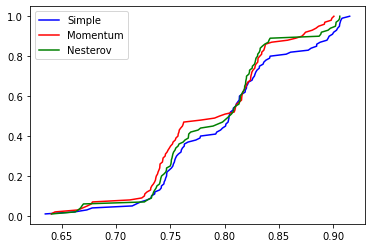
\includegraphics[scale=0.75]{Images/Graphics/simple_momentum_nesterov_100.png}
	\caption{Srovnání algoritmů učení - experiment Hubert}
	Obrázek znázorňuje experimentálně zjištěné distribuční funkce tří pseudo-náhodných veličin,
	a to úspěšností neuronové sítě na testovací sadě natrénované vybraným algoritmem.
	Uvážíme-li že se nenatrénovaná neuronová síť objeví kdesi v parametrickém prostoru,
	a toto její objevení se je pseudo-náhodné, pak to, kam vybraný algoritmus dovede danou neuronovou síť
	v onom parametrickém prostoru, lze brát jako náhodný jev, a tedy úspěšnost neuronové sítě na testovací sadě
	jako náhodnou veličinu.
	Potom lze algoritmy učení porovnávat na základě distribučních funkcí těchto náhodných veličin.
	Prakticky takové porovnání pak proběhne následovně:
	Je-li graf dané distribuční funkce více vpravo, pak daná distribuce je více štědrá
	a naděluje lépe natrénované modely - tedy jí odpovídající algoritmus je v daném nastavení lepší.
	Nyní k tomuto konkrétnímu obrázku:
	Graf označený jako \emph{Simple} znázorňuje výsledky \emph{standardního stochastického gradientního sestupu},
	kde bylo provedeno 5001 iterací, gradient aproximován výpočtem gradientu na dávce o velikosti 30 vzorků,
	řád učení byl $10^{-2}$;
	graf označený jako \emph{Momentum} znázorňuje výsledky \emph{stochastického gradientního sestupu
	za použití hybnosti}, kde bylo provedeno 5001 iterací,
	gradient aproximován výpočtem gradientu na dávce o velikosti 30 vzorků,
	řád učení byl $10^{-3}$ a koeficient $\alpha = 0.9$;
	graf označený jako \emph{Nesterov} znázorňuje výsledky stochastického gradientního sestupu
	za použití \emph{Něstěrovovy hybnosti}, kde bylo provedeno 5001 iterací,
	gradient aproximován výpočtem gradientu na dávce o velikosti 30 vzorků,
	řád učení byl $10^{-3}$ a koeficient $\alpha = 0.9$.
	Všechny tyto výsledky byly dosaženy učením stejného modelu hluboké dopředné neuronové sítě,
	a to na sadě dat MNIST.
	Každá distribuční funkce byla sestavena na základě 100 pozorování.

\end{figure}

\begin{figure}[p] \label{cnn_figure}
	\centering
	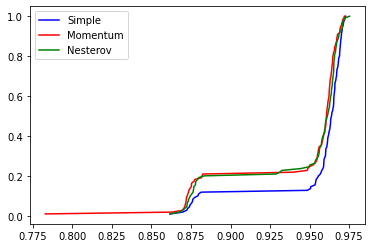
\includegraphics[scale=0.75]{Images/Graphics/simple_momentum_nesterov_cnn_110.png}
	\caption{Srovnání algoritmů učení - experiment Ivan}
	Obdobně jako Obr. \ref{mlp_figure} tento obrázek znázorňuje tři experimentálně zjištěné distribuční funkce.
	Graf označený jako \emph{Simple} znázorňuje výsledky \emph{standardního stochastického gradientního sestupu},
	kde bylo provedeno 5001 iterací, gradient aproximován výpočtem gradientu na dávce o velikosti 30 vzorků,
	řád učení byl $10^{-2}$;
	graf označený jako \emph{Momentum} znázorňuje výsledky \emph{stochastického gradientního sestupu
	za použití hybnosti}, kde bylo provedeno 5001 iterací,
	gradient aproximován výpočtem gradientu na dávce o velikosti 30 vzorků,
	řád učení byl $10^{-3}$ a koeficient $\alpha = 0.9$;
	graf označený jako \emph{Nesterov} znázorňuje výsledky stochastického gradientního sestupu
	za použití \emph{Něstěrovovy hybnosti}, kde bylo provedeno 5001 iterací,
	gradient aproximován výpočtem gradientu na dávce o velikosti 30 vzorků,
	řád učení byl $10^{-3}$ a koeficient $\alpha = 0.9$.
	Všechny tyto výsledky byly dosaženy učením stejného modelu konvoluční neuronové sítě,
	a to na sadě dat MNIST.
	Každá distribuční funkce byla sestavena na základě 110 pozorování.
\end{figure}


% Adversariální vzorky
\chapter{Adversariální vzorky}

\section{Metody generování adversariálních vzorků}

\subsection{FGSM}

\subsection{Iterativní FGSM}


% Robustní učení
\chapter{Robustní učení neuronové sítě}


\pagestyle{headings}

\chapter*{Závěr}

\pagestyle{plain}

\addcontentsline{toc}{chapter}{Záv\v{e}r}

Text závěru....
\begin{thebibliography}{1}
\bibitem{Goodfellow}I. Goodfellow, Y. Bengio, A. Courville,
\emph{Deep Learning}. MIT Press, 2016.

\bibitem{GoodfellowEtAl} I. Goodfellow, J. Shlens, C. Szegedy,
\emph{Explaining and Harnessing Adversarial Examples}. In 'International Conference on Learning Representations', ICLR 2015.

\bibitem{NumericalOptim} J. Nocedal, S. Wright,
\emph{Numerical optimization}. Springer Science \& Business Media, 2006.

\bibitem{Nielsen}M. A. Nielsen, 
\emph{Neural Networks and Deep Learning}. Determination Press, 2018.

\end{thebibliography}

\end{document}
